%\documentclass[a4paper]{report}
\documentclass[a4paper]{article}

%% Language and font encodings



%% Sets page size and margins
\usepackage[a4paper,top=3cm,bottom=2cm,left=3cm,right=3cm,marginparwidth=3cm]{geometry}

%% Useful packages
\usepackage{amsmath}
\usepackage{graphicx}
\usepackage[colorinlistoftodos]{todonotes}
\usepackage[colorlinks=true, allcolors=blue]{hyperref}
\usepackage{subfig}
\usepackage{float}

\usepackage{csquotes}

%\setlength{\tabcolsep}{0pt}

% Write the title here
\title{Pattern Recognition\\
	Assignment 4\\
	Group No - 36 }
\author{ED13D000 Bhargava Sai Ramu\\
	CS17S008 Nitesh Methani}

\begin{document}
\maketitle
\hypersetup{linkcolor=black}
\tableofcontents

% Objectives
\section{Objectives}
\begin{enumerate}
	\item Recognize Digits : Given the MFCC feature vector of a digit uttered by a speaker, classify it as 1, 2 or 3 using HMM and DTW.
	\item Recognize hand written Telugu characters : Given the X and Y coordinates of a Telugu character written by someone, recognize it as 'a', 'ta' or 'da'.
\end{enumerate}

\section{Hidden Markov Model}
\subsection{Isolated Digits}
Table \ref{table:1} is the summary of class wise accuracy of digits 1, 2, 3 for different number of states and symbols.

\hspace*{-1cm}\begin{table}[h]
	\centering
	\begin{tabular}{|l|l|l|l|l|}
		\hline

\textbf{Symbols} & \textbf{States} & \textbf{1} & \textbf{2} & \textbf{3} \\		\hline		\hline
16               & 6               & 100\%          & 100\%          & 97\%       \\		\hline
16               & 4               & 100\%          & 100\%          & 97\%       \\		\hline
16               & 2               & 100\%         & 57\%      & 97\%       \\		\hline
10               & 6               & 100\%          & 97\%       & 93\%       \\		\hline
10               & 4               & 97\%       & 97\%      & 90\%        \\		\hline
10               & 2               & 100\%         & 97\%       & 90\%        \\		\hline
6                & 6               & 100\%         & 97\%      & 90\%        \\		\hline
6                & 4               & 100\%        & 97\%       & 97\%      \\		\hline

\end{tabular}\hspace*{-1cm}
\caption{Digits Class wise Accuracy}
\label{table:1}
\end{table}
\begin{figure}[h!]
	\hspace*{0cm}\begin{tabular}{cc}
		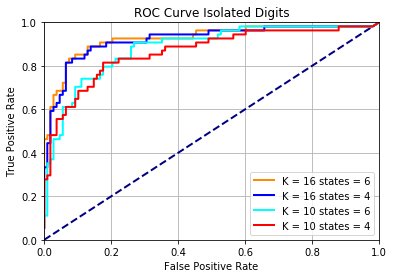
\includegraphics[width=70mm]{HMM/roc_isolated_digit_multiple_Ks.png} & 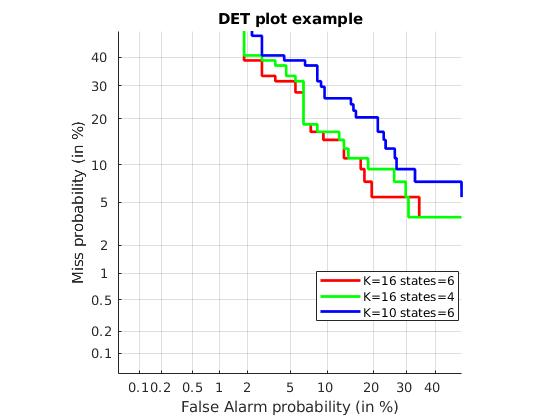
\includegraphics[width=70mm]{HMM/nit_digit_dtw.jpg} \\
		(a) ROC Curve for K=16, Q=6 & (b) DET Curve\\[4pt]
		
	\end{tabular}\hspace*{0cm}
	\caption{Plots for Isolated Digits }
\end{figure}

\newpage
\subsection{Connected Digits}
Table \ref{table:2} is the prediction of our model for the given test data. Initially we had 3 HMM models for 3 digits. We concatenated them with different permutations to get 27 different HMM models. We didn't use dummy state. We modified the transition probabilities of the last state of the individual models such that probability to remain in that state is 0.5 and probability to transit to first state of the next model is also 0.5. The symbol emission probabilities were adjusted accordingly.
\begin{table}[h!]
\centering

\begin{tabular}{|c|c||c|c|}\hline
\textbf{Test 1} & \textbf{Predicted} & \textbf{Test 2(files)} & \textbf{Predicted} \\\hline\hline
11322a            & d2\_d3\_d2\_       & 342 & d2\_d2\_d1\_  \\\hline
132a              & d3\_d2\_d1\_       & 343 & d3\_d2\_d1\_  \\\hline
13a               & d3\_d2\_d2\_       & 344 & d1\_d3\_d1\_  \\\hline
212a              & d2\_d1\_d1\_       & 345 & d1\_d2\_d1\_  \\\hline
21a               & d2\_d1\_d2\_       & 346 & d3\_d1\_d2\_   \\\hline
22123a            & d3\_d3\_d2\_       & 347 & d3\_d2\_d1\_  \\\hline
22a               & d2\_d2\_d1\_       & 348 & d1\_d3\_d1\_  \\\hline
233a              & d2\_d2\_d2\_       & 349 & d1\_d2\_d1\_  \\\hline
23a               & d1\_d1\_d1\_       & 350 & d3\_d1\_d2\_  \\\hline
311a              & d1\_d1\_d2\_       & 351 & d1\_d2\_d2\_  \\\hline
31a               & d1\_d1\_d3\_       & 352 & d1\_d1\_d2\_  \\\hline
322a              & d1\_d2\_d1\_       & 353 & d2\_d1\_d2\_  \\\hline
331a              & d1\_d2\_d2\_       & - & -  \\\hline
33a               & d3\_d1\_d2\_       & - & -  \\\hline
\end{tabular}
\caption{Connected Digits Recognition}
\label{table:2}
\end{table}



\section{Recognition of Hand Written data}
\subsection{Feature Extraction}
Size Normalization:
Size of the characters varies from writer to writer due to different writing styles. Therefore to make all the samples of uniform size we did size normalization to improve the recognition performance. Now the character data are normalized to fit into a box of unit length.
Other features extracted are as follows:
\begin{enumerate}
	\item Features
	\begin{enumerate}
		\item Normalized Coordinate Values : Normalized X and Y coordinates are used as features.
		Reason : They represent the shape of the character in abstract format.
		
		\item Deviation Features : Characters vary in size and shape with the variation in character trajectories either in horizontal or vertical directions. So deviation features are extracted.
		
		\item Zero Mean Feature : Distance of the horizontal and vertical coordinate values from the horizontal and vertical means is calculated. Since data points are subtracted from the data mean, the resulting data is named as Zero mean features.
		
		\item Trajectory Features : While writing a character handwriting forms a trajectory which comprises of angle and distance parameters.
		Distance and angle parameter from the origin of the Cartesian Coordinate System and the horizontal axis respectively.
		Distance and angle parameter from the centroid.
		Distance and angle parameter between the consecutive points.
	\end{enumerate}
	\item Other Features
	\begin{enumerate}
		\item Curvature
		\item Cosine Distances
		\item Slope
		\item First Derivative
		\item Second Derivative
		\item Normalized First Derivative
		\item Normalized Second Derivative
	\end{enumerate}
\end{enumerate}
The values in the extracted feature are normalizd to fit in a window size of [0, 1].






\subsection{Isolated Handwritten Characters}
Table \ref{table:3} is the summary of class wise accuracy of handwritten characters a, dA, tA for different number of states and symbols.

\hspace*{-1cm}\begin{table}[h]
\centering
\begin{tabular}{|l|l|l|l|l|}
	 \hline
\textbf{Symbols} & \textbf{States} & \textbf{a} & \textbf{dA} & \textbf{tA} \\ \hline \hline
16               & 6               & 100\%          & 94\%        & 100\%           \\ \hline
16               & 4               & 100\%         & 94\%        & 100\%      \\ \hline
16               & 2               & 100\%         & 94\%        & 100\%           \\ \hline
10               & 6               & 94\%      & 100\%           & 100\%          \\ \hline
10               & 4               & 89\%       & 94\%        & 100\%        \\ \hline
10               & 2               & 89\%       & 89\%        & 100\%           \\ \hline
6                & 6               & 94\%       & 94\%      & 94\%        \\ \hline
6                & 4               & 94\%       & 83\%        & 100\%           \\ \hline
6                & 2               & 94\%       & 89\%        & 100\%           \\
 \hline
\end{tabular}\hspace*{-1cm}
\caption{Handwritten Characters Class wise Accuracy}
\label{table:3}
\end{table}
\begin{figure}[h!]
	\hspace*{0cm}\begin{tabular}{cc}
		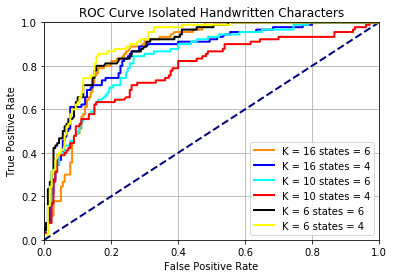
\includegraphics[width=70mm]{HMM/roc_handwritten_multiple_Ks.png} & 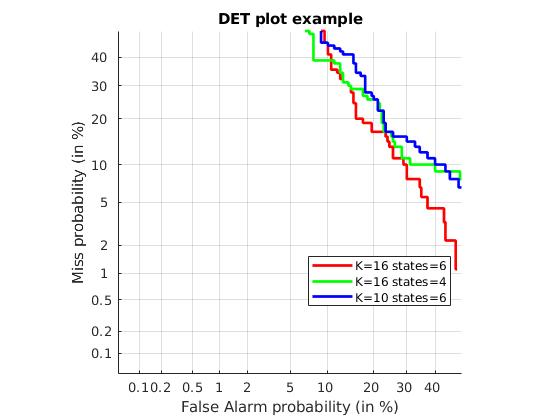
\includegraphics[width=70mm]{HMM/nit_char_dtw.jpg} \\
		(a) ROC Curve & (b) DET Curve\\[4pt]
		
	\end{tabular}\hspace*{0cm}
	\caption{Plots for Isolated Handwritten Characters}
\end{figure}

\subsection{Connected Handwritten Characters}
Table \ref{table:4} is the prediction of our model for the given test data. Initially we had 3 HMM models for 3 characters. We concatenated them with different permutations to get 27 different HMM models. We didn't use dummy state. We modified the transition probabilities of the last state of the individual models such that probability to remain in that state is 0.5 and probability to transit to first state of the next model is also 0.5. The symbol emission probabilities were adjusted accordingly.
\begin{table}[h!]
\centering

\begin{tabular}{|c|c|}\hline

Given Characters & Predicted\\ \hline\hline
dA tA dA & tA tA a \\ \hline
dA tA a & a tA a \\ \hline
dA dA dA & a dA a \\\hline

\end{tabular}
\caption{Connected Handwritten Characters Recognition}
\label{table:4}
\end{table}



\newpage
\section{Dynamic Time Warping}
\subsection{Observations}
Table \ref{table:5} is the summary of accuracy of normalized and raw data using brute force and representative method.

\hspace*{-1cm}\begin{table}[h]
	\centering
	\begin{tabular}{|l|l|l|l|l|}

\hline
DTW & Accuracy & Time \\ \hline\hline
Raw Data & 100\% & 00:11:53:41 \\ \hline
Zero-mean              &   38.89\%  & 00:09:32:57 \\ \hline
Min-Max Normalization  &   42.52\%  & 00:09:44.80 \\ \hline
Using Representatives  &  98.84\%   & 00:01:49:37 \\ \hline
Vector Quantization    &   48.14\%  & 00:11:38.18 \\ \hline

		
	\end{tabular}\hspace*{-1cm}
	\caption{Recognition Rates}
	\label{table:5}
\end{table}
\subsection{Observations}
\begin{figure}[h!]
	\hspace*{1cm}\begin{tabular}{cc}
		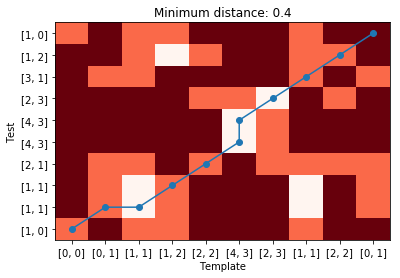
\includegraphics[width=70mm]{DTW/dtw_try.png} & 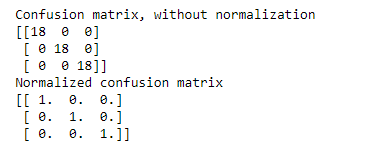
\includegraphics[width=70mm]{DTW/confusion_matrix_raw_data.png} \\
		(a) Example DTW & (b) Confusion Matrix on Raw Data\\[4pt]
		
		% To plot 5 images i 3x2 table
		\multicolumn{2}{c}{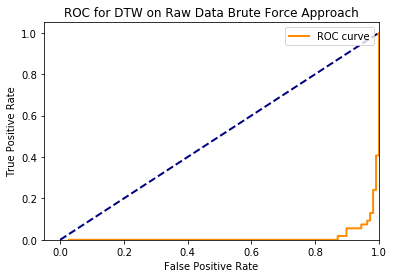
\includegraphics[width=70mm]{DTW/roc_dtw.png} }\\
		\multicolumn{2}{c}{(c) ROC Curve}
		
	\end{tabular}\hspace*{1cm}
	\caption{Plots for DTW}
\end{figure}
Representatives are as follows:\newline
Class 1 : $30^{th}$ and $31^{st}$ template\newline
Class 2 : $31^{st}$ and $22^{nd}$ template\newline
Class 3 : $15^{th}$ and $8^{th}$ template
\newpage
\section{Coding Style Improvement}
\begin{itemize}
  \item Writing Object Oriented Code for re-usability.
  \item Writing shell scripts to avoid writing commands again and again on the terminal.
  \item Added modularity while writting code.
  \item Practiced multi-file programming style and some regular expressions for file handing.
  \item Better handling images and tables in latex.
\end{itemize}
\section{Conclusion}
In this assignment we generated HMM models for different number of symbols and states and trained them on digits 1, 2 and 3 and characters a, tA and dA for the respective questions. After testing them independently we then connected them to recognize the connected strings. We also did the recognition task using DTW method. One of the mistakes that we were doing was to do K-Means on the test data again for assigning cluster labels.
\end{document}